\section{Polarimeter Dermoscope}
\label{sec:chp5-sec2}
Figures~\ref{fig:internal-des} and \ref{fig:dermo-polar-des} show the internal design of the polarimeter dermoscope and our first prototype, respectively.
This dermoscope consists of several different parts: a camera, a lense, a focusing mechanism, a \ac{psg} and \ac{psa} units, and an electronic controller.
This system provides configurable acquisitions allowing for the adjustment of different parameters, including the number of acquisitions and polarization angles in both the \ac{psg} and \ac{psa} units.
The desired configuration can be set via a USB connector.

\begin{figure}
	\begin{center}
		\subfloat[]{\label{fig:internal-des1}
			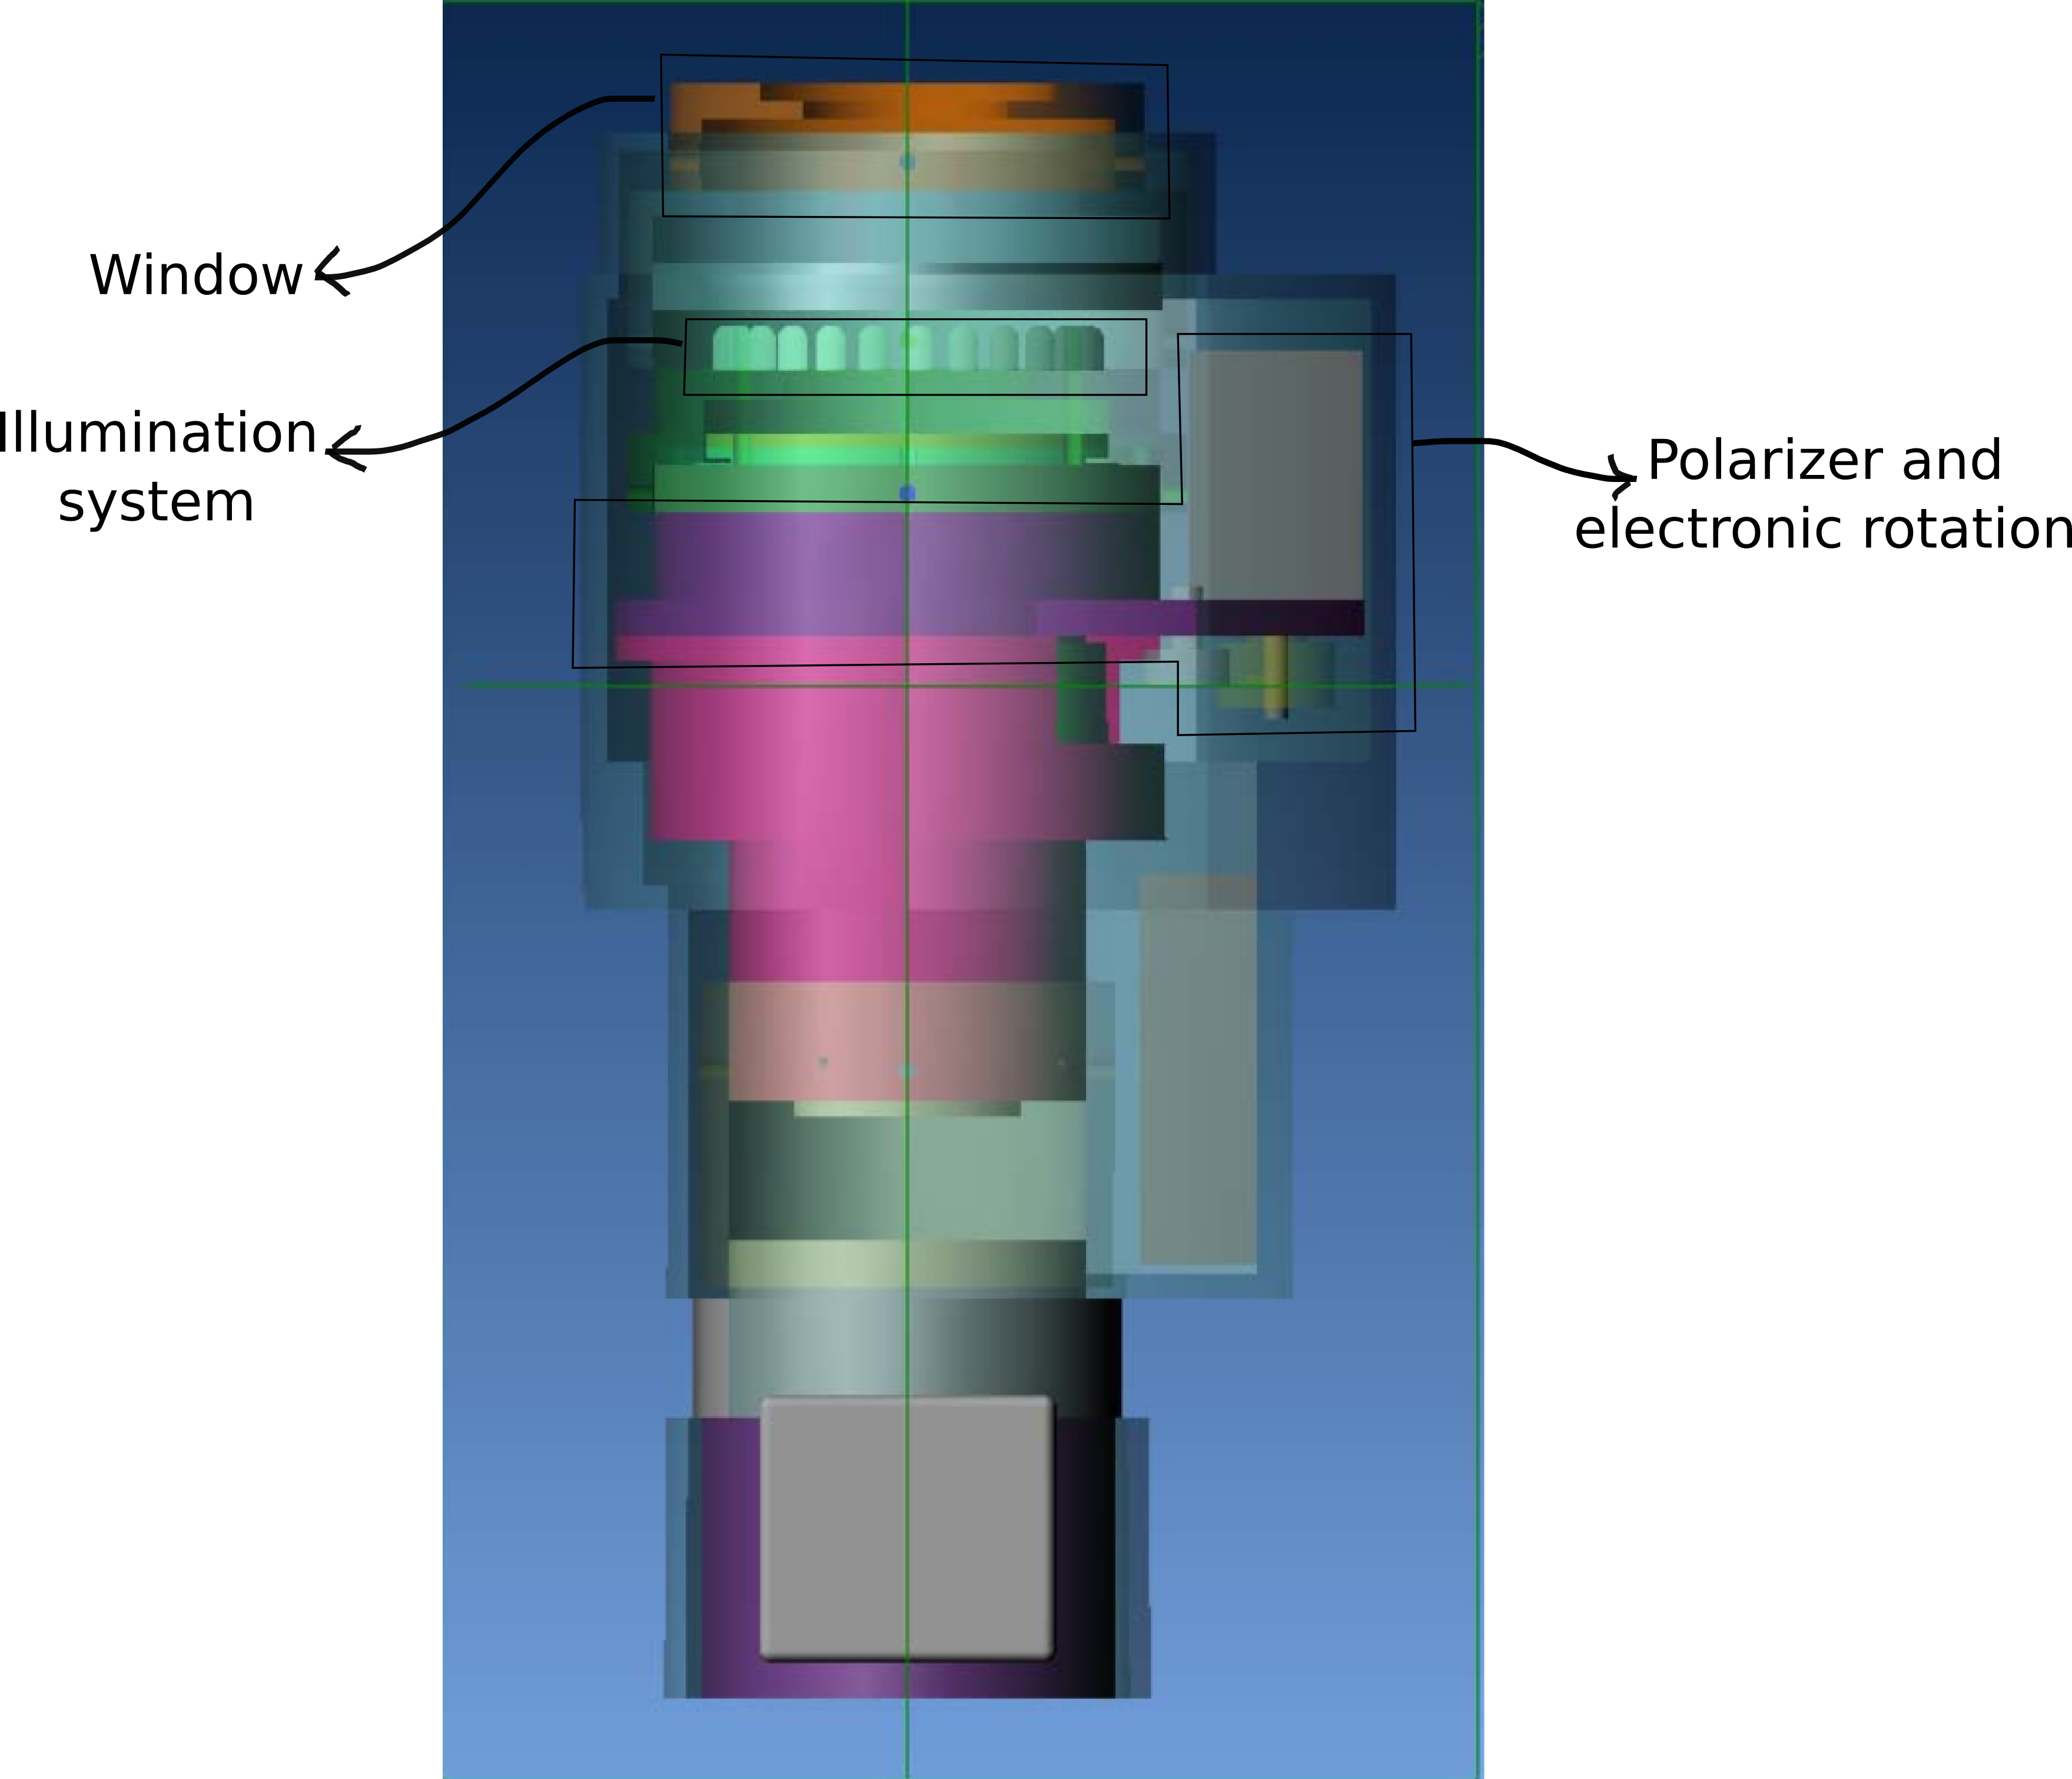
\includegraphics[width = 0.8\textwidth]{Chapter5/Figures/PD-1-modified.png}}\\		
		\subfloat[]{\label{fig:internal-des2}
			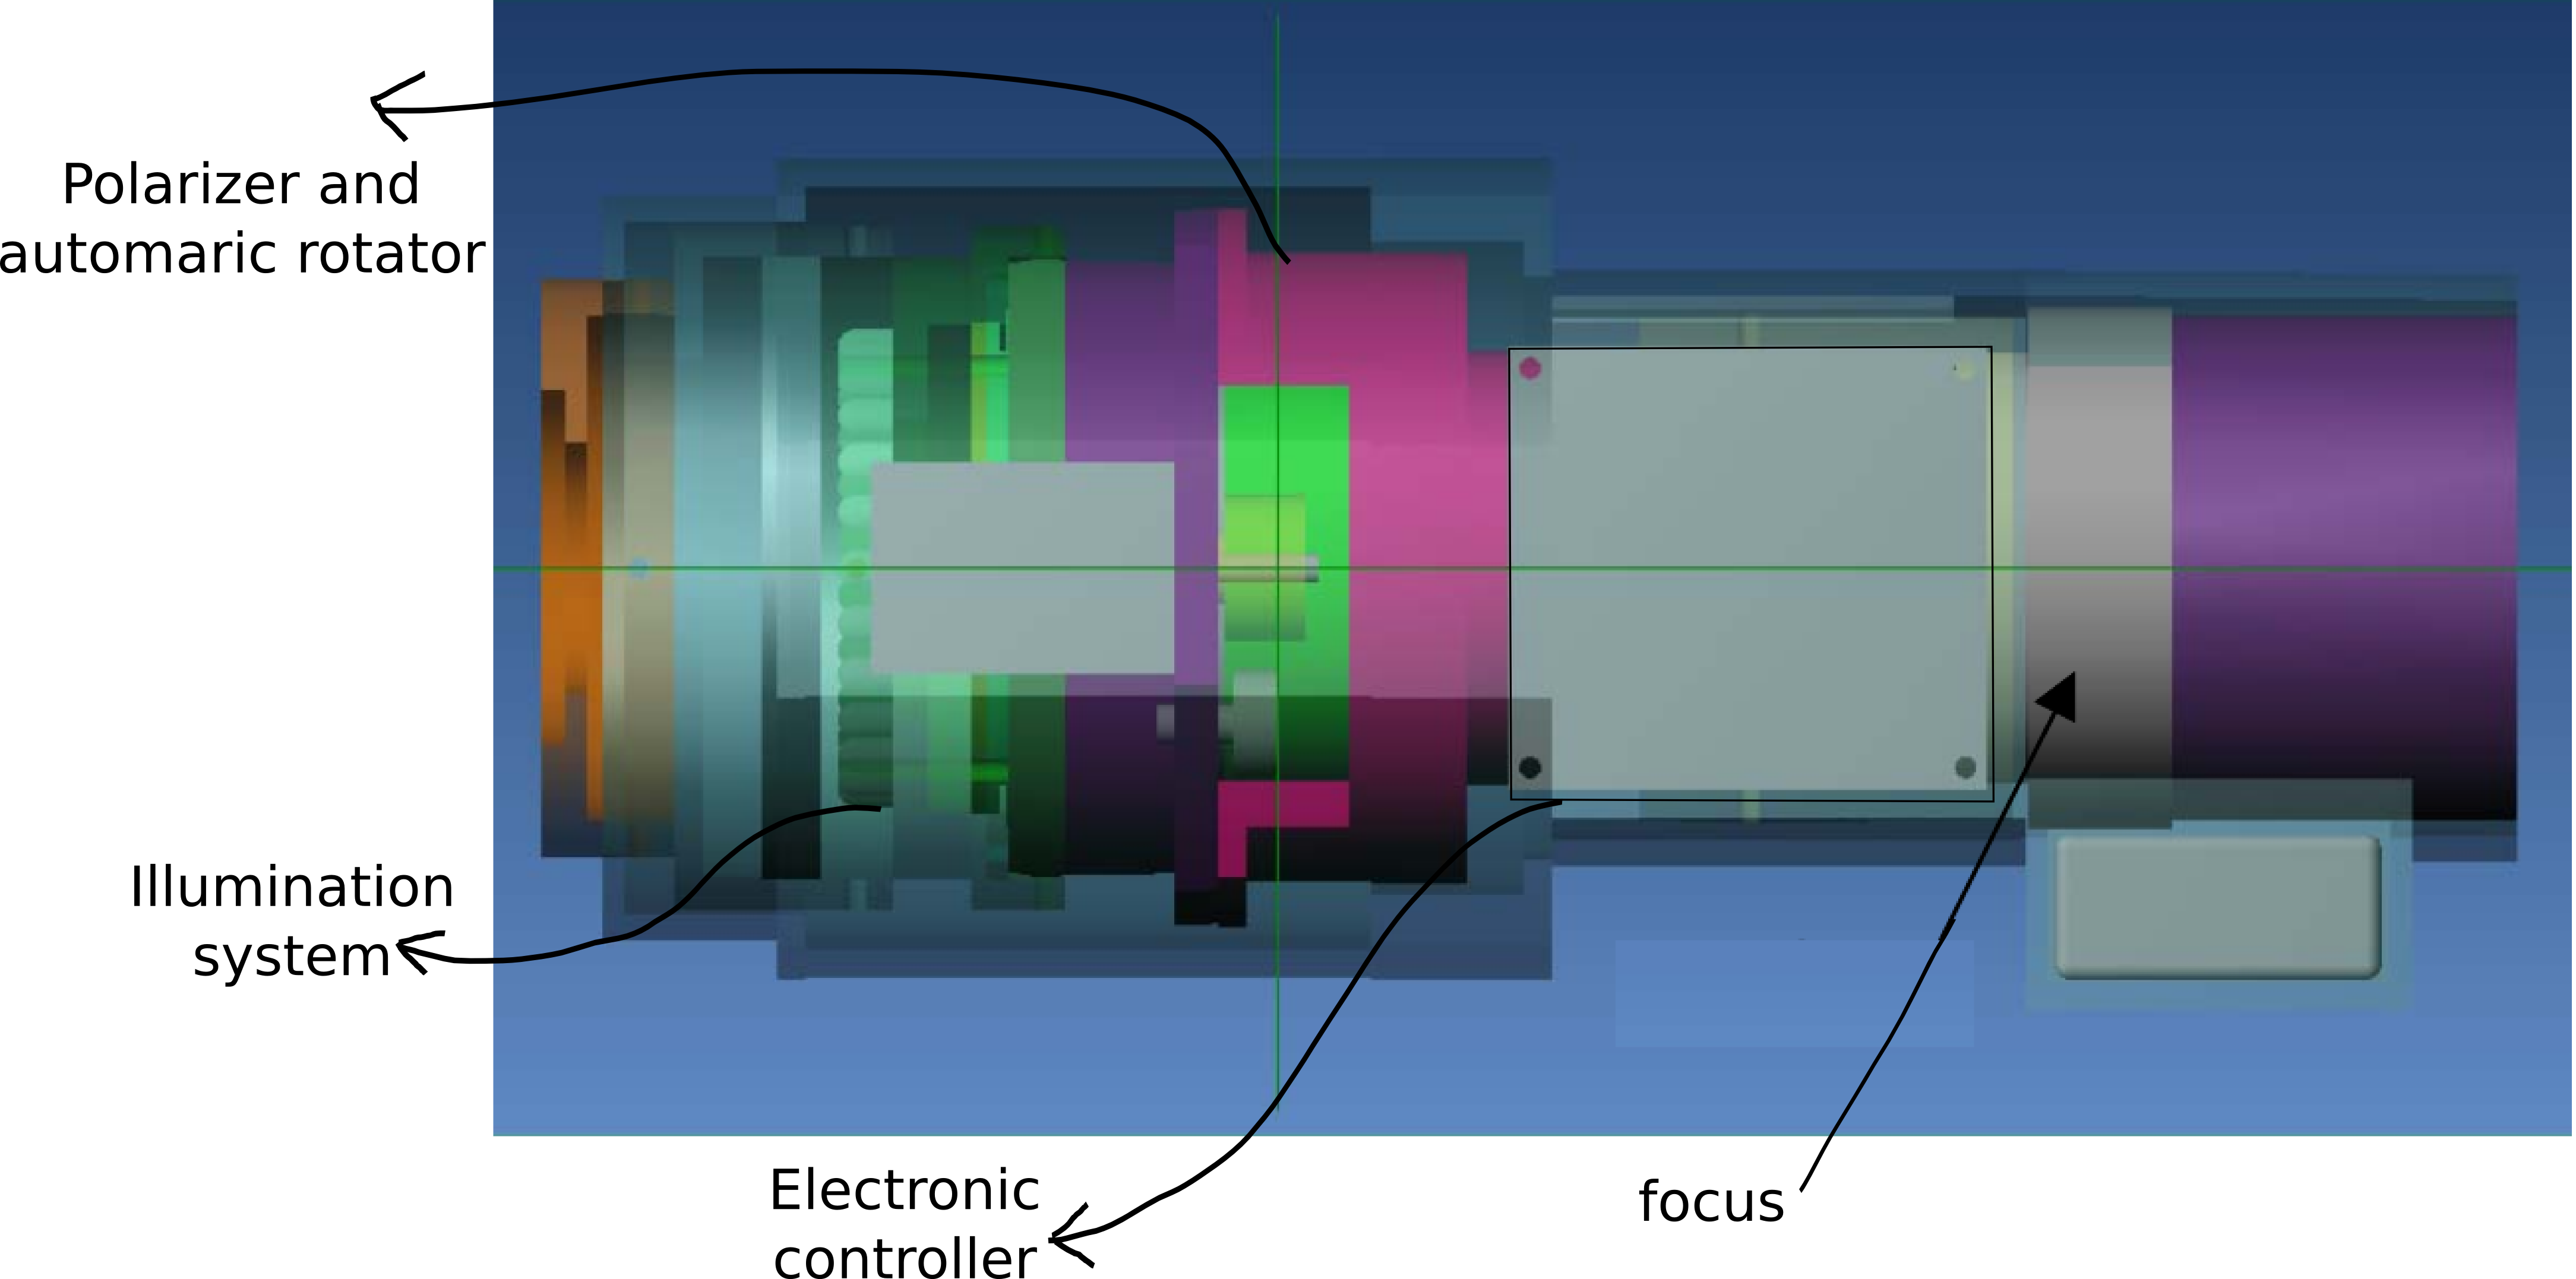
\includegraphics[width = 0.8\textwidth]{Chapter5/Figures/PD-2-modified.png}}
	\end{center}
	\caption[Internal design of polarimeter dermoscope]{Internal design of the polarimeter dermoscope.}
	\label{fig:internal-des}
\end{figure}

\begin{figure}
	\begin{center}
		\subfloat[]{\label{fig:dermo-polar-des1}
			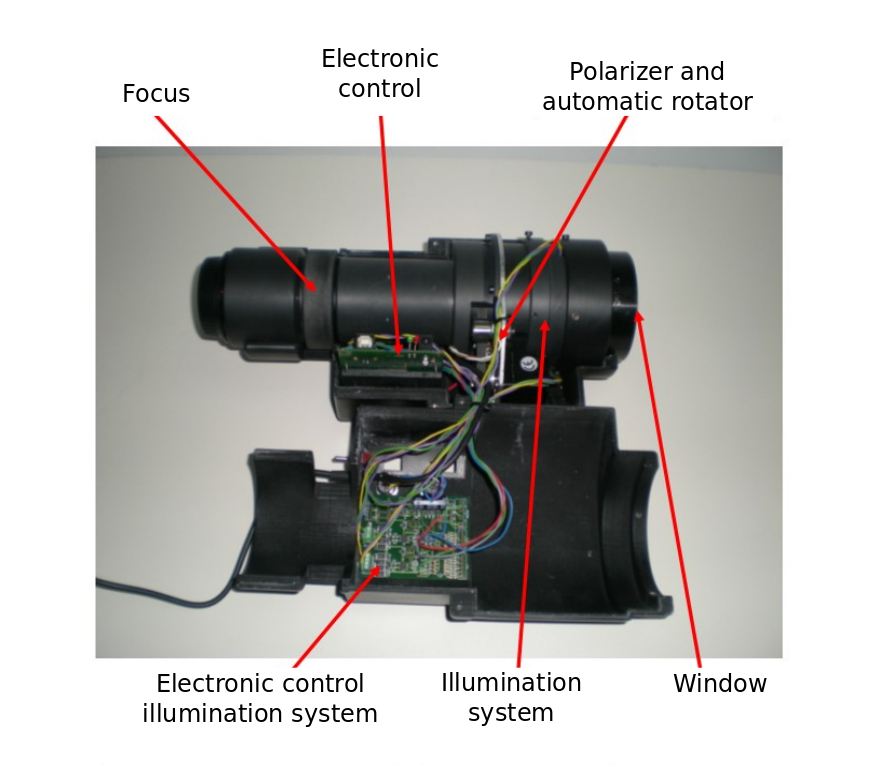
\includegraphics[width = 0.7\textwidth]{Chapter5/Figures/PD-3-modified.png}}\\
		\subfloat[]{\label{fig:dermo-polar-des2}
			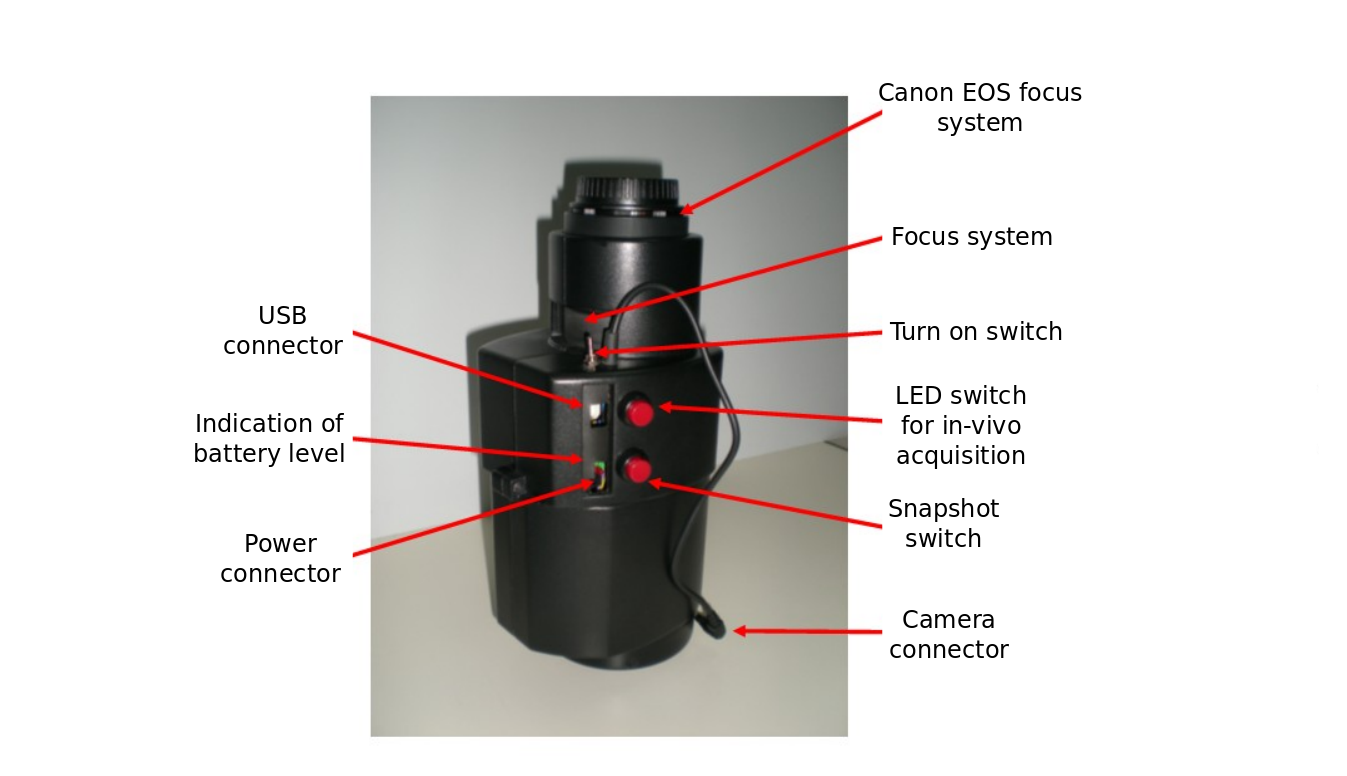
\includegraphics[width = 1.1\textwidth]{Chapter5/Figures/PD-4-modified.png}}
	\end{center}
	\caption[The first prototype of polariemeter dermoscope]{Polarimeter dermoscope first prototype.}
	\label{fig:dermo-polar-des}
\end{figure}

The system is designed to fit the distance sensor and the coupling mechanism in any of the Canon EOS models.
Its focusing system placed right after the camera coupling mechanism, is manual.
As shown in Fig.\ref{fig:dermo-polar-des1}, the device has a switch and two buttons. 
The switch turns the device on and off while the buttons are for controlling the acquisition.
The first button lights up the illumination system and allows visualization of the acquisition in-vivo using a liveview approach.
The second button starts the acquisition process.

This polarimetric dermoscope has three connectors: (i) the connector for the signal exchange with the camera, (ii) the USB connector, and (iii) the power supply connector.
The USB connector is used to set an automatic image acquisition program, while the power supply connector serves to charge the dermoscope for autonomous use.
The optical system of the \ac{psa} unit consists of a dermoscope with a fixed macro lens, Schneider Componon-S 4.0/80, which has the magnifier with ratio of 1 (1:1).
The lens is followed by a polarizer with a rotating system driven by a stepper motor programmable via the USB connector.

The \ac{psg} unit consists of a ring of white LEDs (model: Cree SMD white LED) as the illumination system (Fig.~\ref{fig:LED}).
This system is followed by a diffuser for uniform illumination and a fixed polarizer.
The fixed polarizer is positioned so that the first image is acquired with cross-polarized illumination (the polarizer of the \ac{psa} unit is positioned at \ang{90} with respect to the horizontal axis of the fixed polarizer).
For the image acquisition, the skin lesion should be in contact with the borosilicate window.

\begin{figure}
	\begin{center}
		\subfloat[]{\label{fig:LED}
			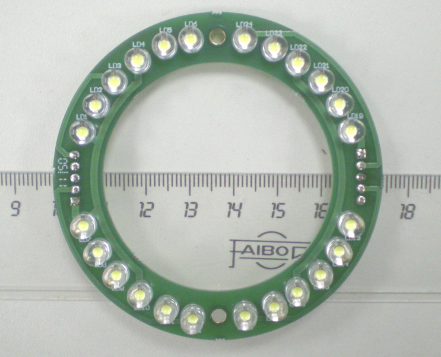
\includegraphics[width = 0.35\textwidth]{Chapter5/Figures/LEDS.png}}
		\subfloat[]{\label{fig:EC}
		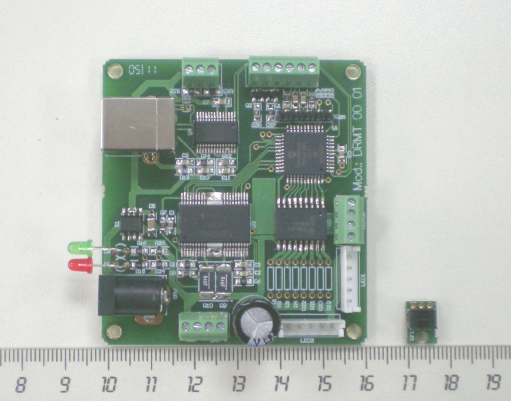
\includegraphics[width = 0.363\textwidth]{Chapter5/Figures/ElectronicController.png}}
	\end{center}
	\caption[The illumination system and electronic board of the polarimetric dermoscope]{(a) Ring of white LEDs for the illumination system of the \ac{psg} unit. (b) Electronic board of the polarimeter dermoscope.}
	\label{fig:LED_EC}
\end{figure}

The dermoscope's focusing is done manually by rotating the ring placed just after the camera's coupling mechanism, as shown in Figs.\,\ref{fig:dermo-polar-des} and \ref{fig:internal-des2}.
Figure~\ref{fig:EC} shows the board for electronic control, while its position is shown in Fig.\,\ref{fig:internal-des}.

%\begin{figure}
%	\centering
%	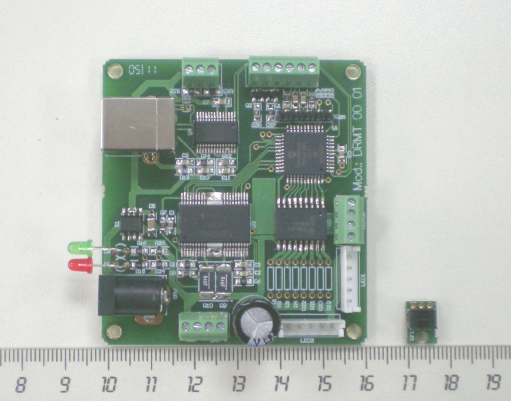
\includegraphics[width = 0.35\textwidth]{Chapter5/Figures/ElectronicController.png}
%	\caption[Electronic board of polarimeter dermoscope]{The Electronic board of the polarimeter dermoscope.}
%	\label{fig:EC}
%\end{figure}


%The target object should be placed in front of the borosilicate window.



